\chapter{Introduction}

\section{Problem Statement}
    % ควรพูดถึงover all problems 
    % 2 main problem 
    
    % Epidemic = ระบาด
    % ------need to re-write------------
    
    % make a policy decision
    Human Immunodeficiency Virus (HIV), Acquired Immune Deficiency Syndrome (AIDS), Tuberculosis (TB), Hepatitis, and Sexually Transmitted Disease (STD) are included as diseases under surveillance that Ministry of Public Health (Thailand) has a responsibility to prevent and control those disease. The main goal of the ministry is to decrease the number of new patients that are infected by diseases under surveillance. According to the Ministry of Public Health (Thailand), the ministry want to reduce the number of TB patient to have less than 60,000 patients per year, and also they want to reduce the number of AIDS patients to be less than 1,000 people per year by 2030. Also, Asean Economics Community (AEC) has a policy to prevent and control epidemic diseases between countries. To prevent and control diseases under surveillance in Thailand, the Ministry of Public Health of Thailand has to surveil and follow the patient who has disease under surveillance. Bureau of Epidemiology is the main institute to surveil by cooperating with other sectors such as hospital, provincial public health, and other sector that will be involved in order to reduce the workload of the staff, who have a responsibility to surveil and follow patients under surveillance report. In order to reduce the workload, they have to work together with sectors under the Ministry of Public Health (Bureau of Epidemiology, Bureau of AIDS TB and STIs, Bureau of Strategy and Policy, Information Technology and Communication Center, Bureau of health promotion, Office of the Permanent Secretary, Department of medical science), sectors under Bangkok ministry (The BMA Health Department, Medical Service Department), and Thailand MOPH-US CDC Collaboration to develop the system to surveil and follow the disease under surveillance in order to make a policy decision.

\section{Problems} \label{section:problems}
    % lists problem 
    There are two main problems that they are facing which are surveil and follow the patient who has disease under surveillance in order to make decision policy and reduce the number of workload of the staff. 
    
    Firstly, they want to surveil and follow the patient who has disease under surveillance in order to prevent and control diseases under surveillance in Thailand. This is the main problem because they cannot surveil and follow all of the patient, they can surveil and follow only the small scope(only in their hospital scope) which led to the problem that they cannot prevent and control diseases under surveillance. In addition, another reason that they follow and monitor those patient is because they also want to make a policy decision. For example, if MOPH want to give a budget to provide to Provincial Public Health, so they will know that which province that they should give more budget on.
    
    Secondly, they want to reduce the number of workload of the staff who surveil and follow the patient who has disease under surveillance. Before having the system, the hospitals had been using the systems called NAP (National AIDS Program)\cite{nap} and NAPDAR (NAP Data Analysis \& Reporting). There are many steps to upload and see the report as you can see the functional of NAP and NAPDAR in section 1.3 Existing Solution. This is another problem because the staff have to do a lot of work in order to see a report.
    
\section{Analyse problem}
    Ministry of Public Health (Thailand) has responsibility to solve all problems in section \ref{section:problems}. However, those problems are very big scope, so we need to analyse and narrow down those problems in order to make policy decision. 
    
    Firstly, they want to be able to get overall status of patient who visit to the hospital and care in Thailand, so we need to create at a glance report. This report will represent the overall number of patients in particular disease that we want, for instance,the amount of people who have particular disease, the amount of drugs that have been use in that year, and so on.
    
        
    Secondly, they want to know the overall number of patients in particular diseases in term of demography that can be separate by several category such as gender, nation, occupation, etc. The solution to solve this problem is to have a demographic report which will represent in term of graph such as pie chart or histogram to show overall number of patients according to their gender or nation or occupation etc.
    
    Thirdly, HIV is one of our main diseases that is under surveillance, and it is the first disease that they want to focus and be able to monitor. In order to check whether that patient is one of HIV patient or not, it needs to have some data from HIV lab result of patients. To achieve this HIV lab result, we need to have upload lab file function. In addition, after upload function was include then it needs to have checking upload function for them to check whether HIV lab was upload or not.
    
    Fourthly, they want to be able to monitor and follow individual patient across all hospital because patients likely to loss from the system as they move hospital or stop visiting hospital. In order to do this, we need to have individual report which will show the time and list of hospital that patient visit as well as the amount of drug they receive, and so on.
    
    Lastly, from the problem of minimising staff's workload, we need the data that can help to measure the workload. At this time, they want to be able to measure only HIV workload. Solution of this problem is to have workload report which will tell how many HIV patients in this hospital and how many drug that was use to those patients.
    
% 1. monitor
%     - report
%     -send file
%     -check upload status
% 2. less work
%     - nap +nap data analy ==> eiis 

\section{Existing Solution}
    
    Before the implementation of our system, Bureau of Epidemiology (under the supervised of Department of Disease Control and Ministry of Public Health) and the hospitals had been using the systems called NAP (National AIDS Program)\cite{nap} and NAPDAR (NAP Data Analysis \& Reporting).
    
    NAP (National AIDS Program) is the web application that is provided by National Health Security Office (NHSO). The main purpose of NAP system is to follow up the HIV and aids patients. The patients identity will be kept by using NAP Number (generated by the NAP system) for referring the patient using the NAP Number instead of the patients name or citizen identification number. Moreover, HIV or AIDs patient will be registered into the system only once. The next time the patient changes the hospital to visit, NAP system can still retrieve the record of that patient for the treatment. There are 6 roles of user that can access the NAP system. First; HIV-Coordinator, can see the VTC (Voluntary Counseling and Testing), the registration, the lab result, the patients follow up (how many patients that still come and receiving the drug), the change of medicine within their service location. Second; doctor of the patient, has the same authorization as the HIV-Coordinator but cannot add, edit, or modify the record. Third, specialist doctor for medicine change approval; can see the approval of medicine change menu and he/she must be appointed by National Health Security Office. Fourth, pharmacist; can see the Stock Medicine Management and can add, delete, or edit the record in the stock medicine management. Fifth, laboratory technician staff; can only access the lab result menu and sending patient form. Finally, advisors; can see the VTC menu.
    
    NAPDAR (NAP Data Analysis \& Reporting) is the desktop application that is also provided by National Health Security Office. It is the extension from NAP. It is the application for analysing and generating the report from the given data from NAP application. The way NAPDAR works is that the user needs to download the set of data from NAP. Each data is the record of each patient. Then, the user needs to login to NAPDAR and upload the data to the NAPDAR one by one in order to see the report.
    
    % insert NAPDAR pictures
    \FloatBarrier
	\begin{figure}[h!]
        \centering
    		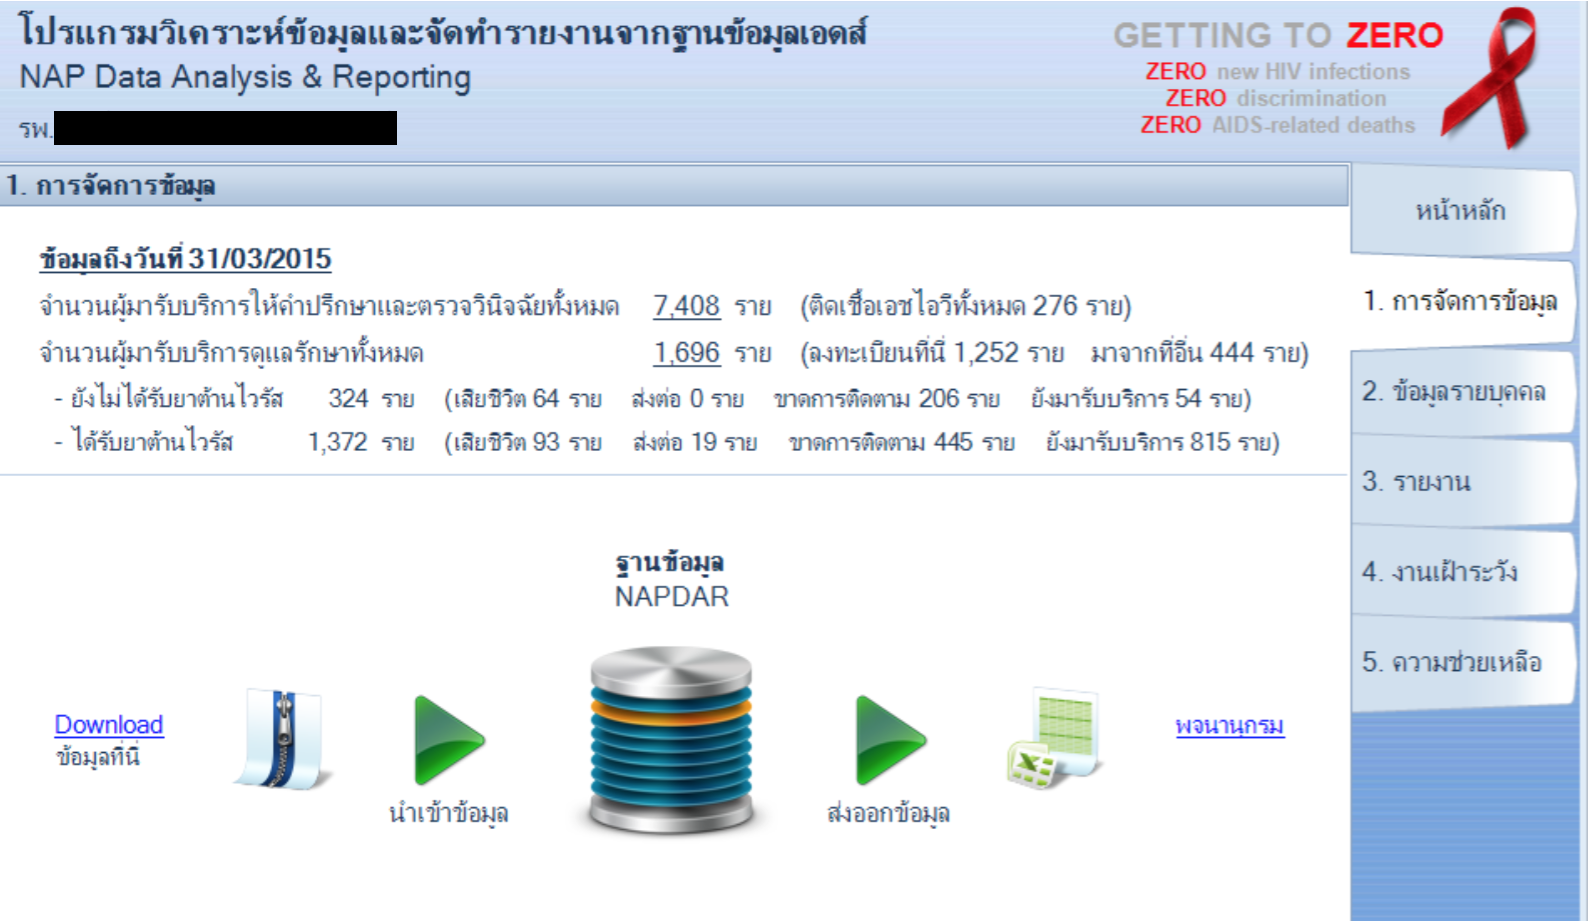
\includegraphics[width=12cm]{images/chapter-01/napdar-01.png}
    		\caption{NAPDAR Data Management Page}
    \end{figure}
\FloatBarrier

\FloatBarrier
	\begin{figure}[h!]
        \centering
    		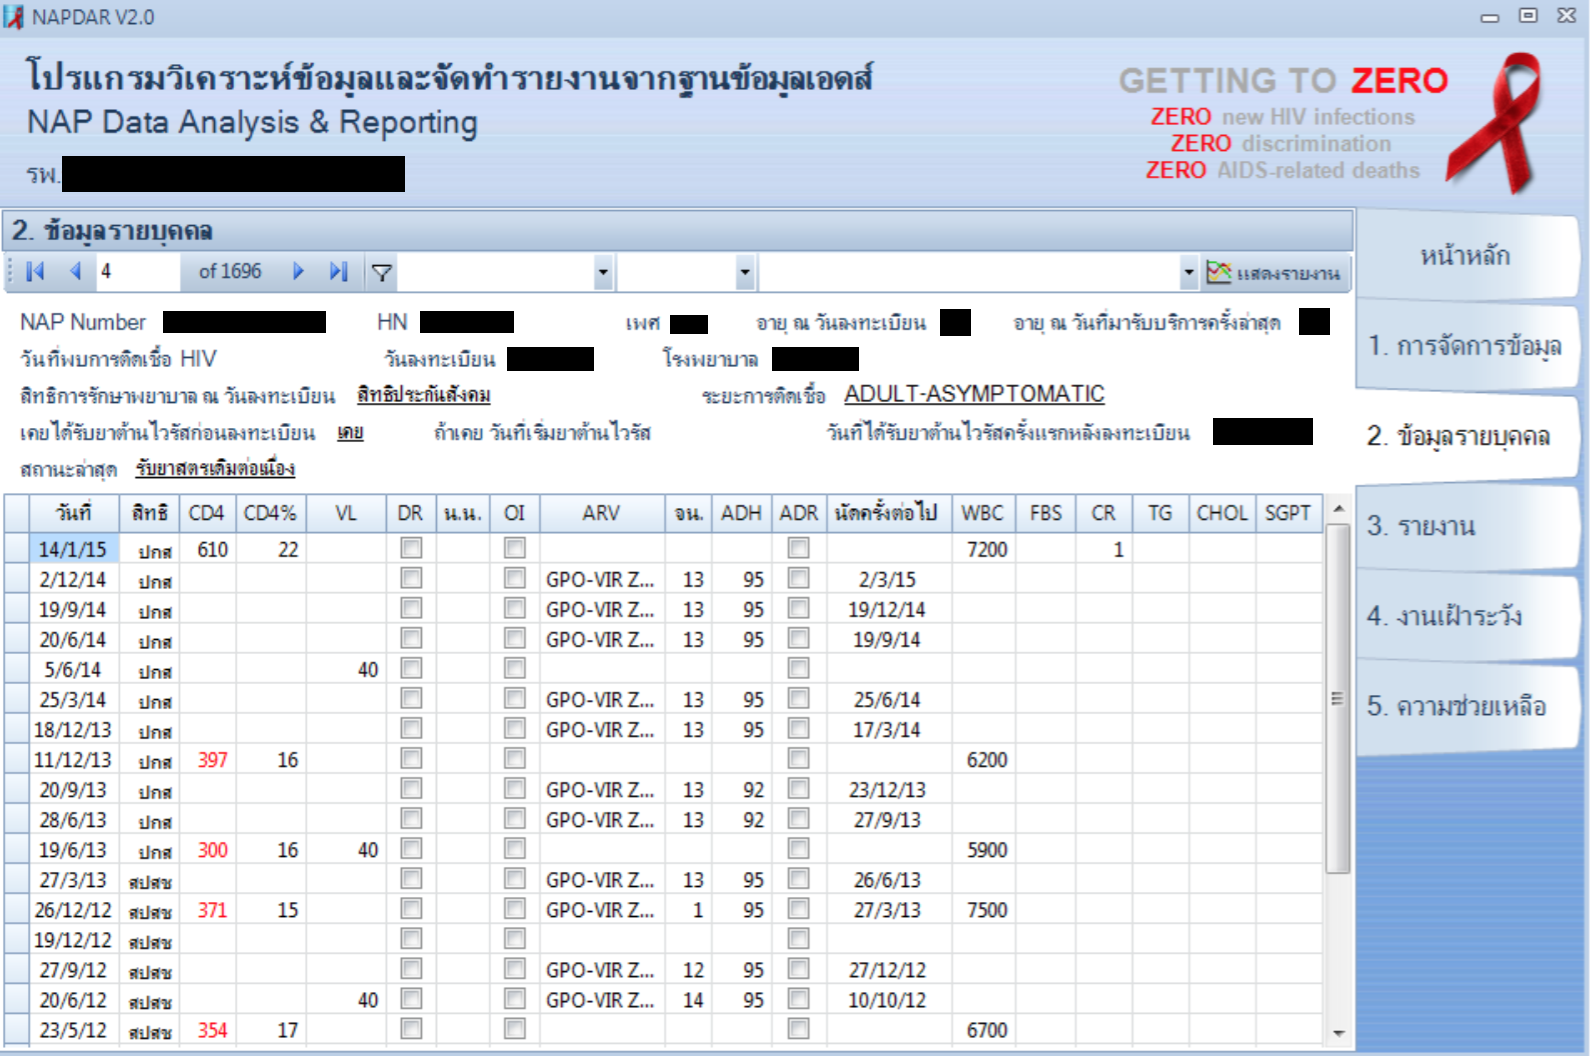
\includegraphics[width=12cm]{images/chapter-01/napdar-02.png}
    		\caption{NAPDAR Individual Report Page}
    \end{figure}
\FloatBarrier

\FloatBarrier
	\begin{figure}[h!]
        \centering
    		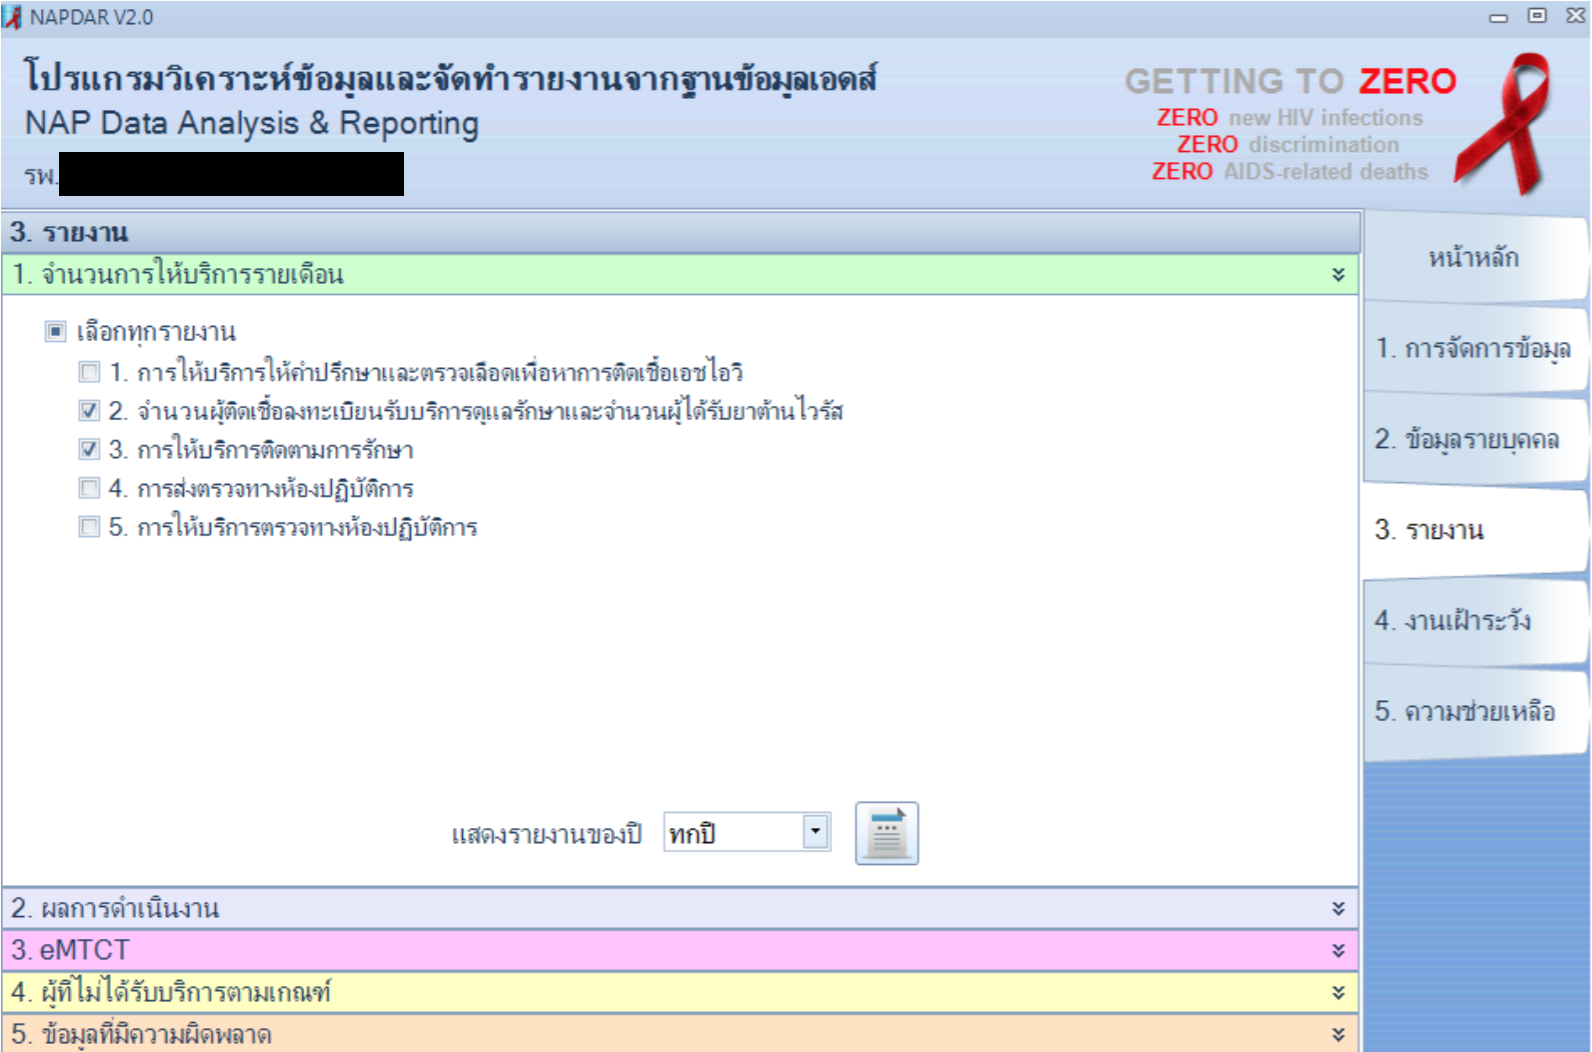
\includegraphics[width=12cm]{images/chapter-01/napdar-03.png}
    		\caption{NAPDAR Generating Monthly Report Page}
    \end{figure}
\FloatBarrier

% \FloatBarrier
% 	\begin{figure}[h!]
%         \centering
%     		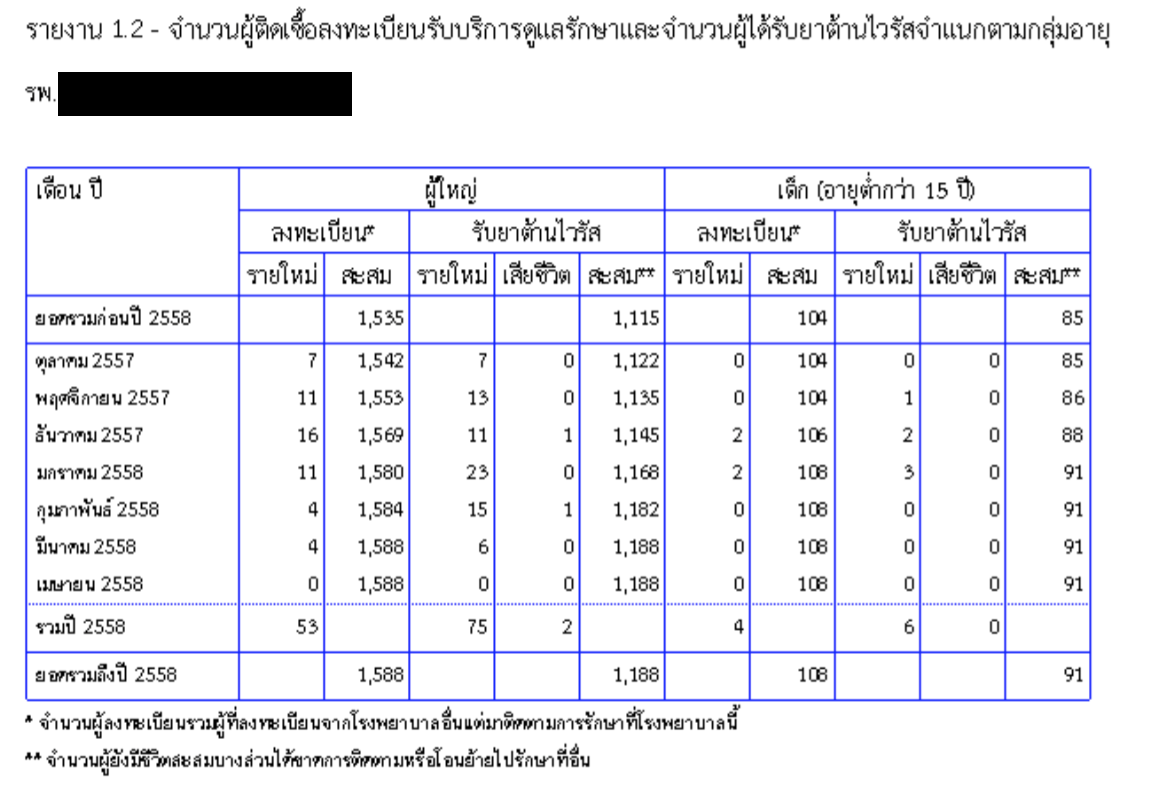
\includegraphics[width=12cm]{images/chapter-01/napdar-04.png}
%     		\caption{NAPDAR Report 1.2}
%     \end{figure}
% \FloatBarrier

\FloatBarrier
	\begin{figure}[h!]
        \centering
    		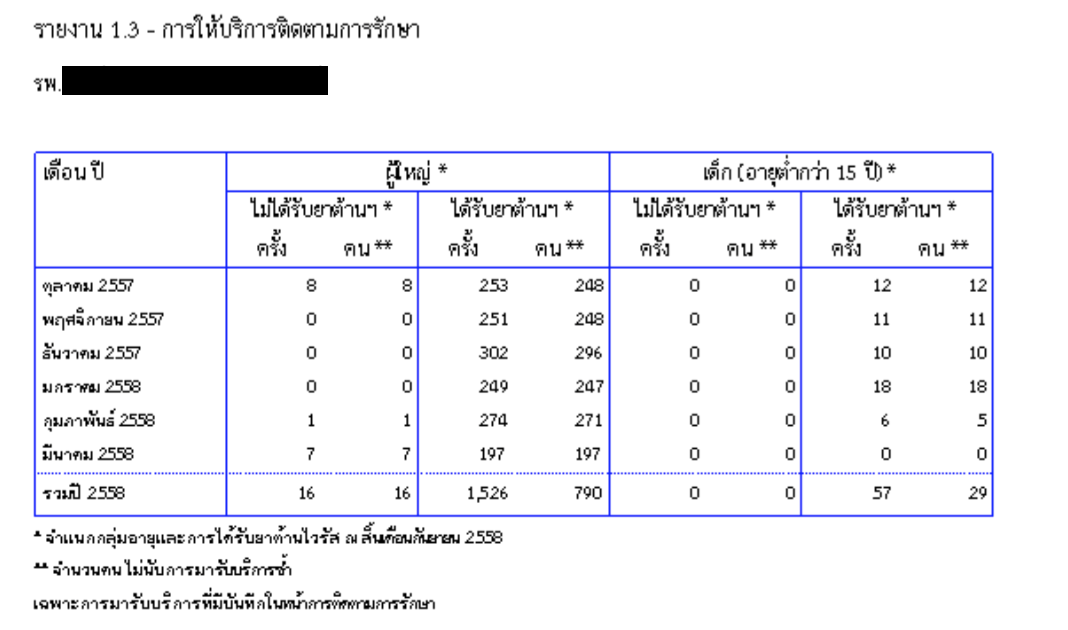
\includegraphics[width=12cm]{images/chapter-01/napdar-05.png}
    		\caption{NAPDAR Follow Up Patient Report}
    \end{figure}
\FloatBarrier

% \FloatBarrier
% 	\begin{figure}[h!]
%         \centering
%     		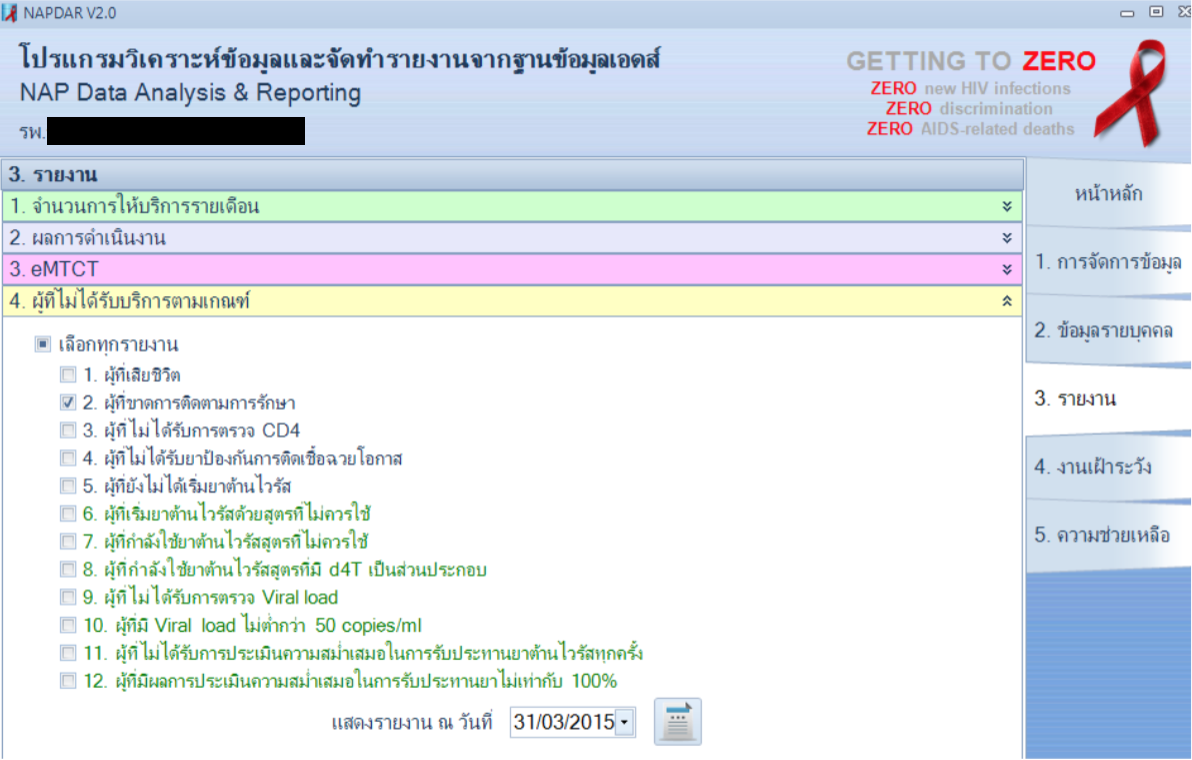
\includegraphics[width=12cm]{images/chapter-01/napdar-06.png}
%     		\caption{NAPDAR Untreated Patient Report Page}
%     \end{figure}
% \FloatBarrier

% \FloatBarrier
% 	\begin{figure}[h!]
%         \centering
%     		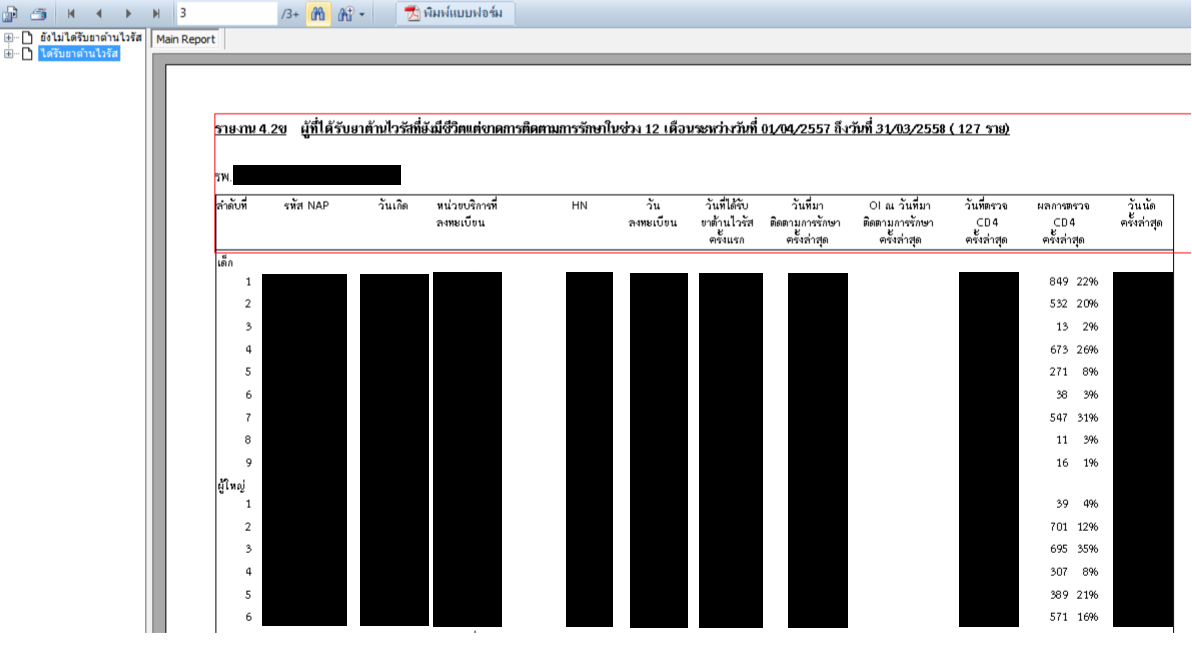
\includegraphics[width=12cm]{images/chapter-01/napdar-07.png}
%     		\caption{NAPDAR Treated Patient with Lost Follow Up Report Page}
%     \end{figure}
% \FloatBarrier

\FloatBarrier
	\begin{figure}[h!]
        \centering
    		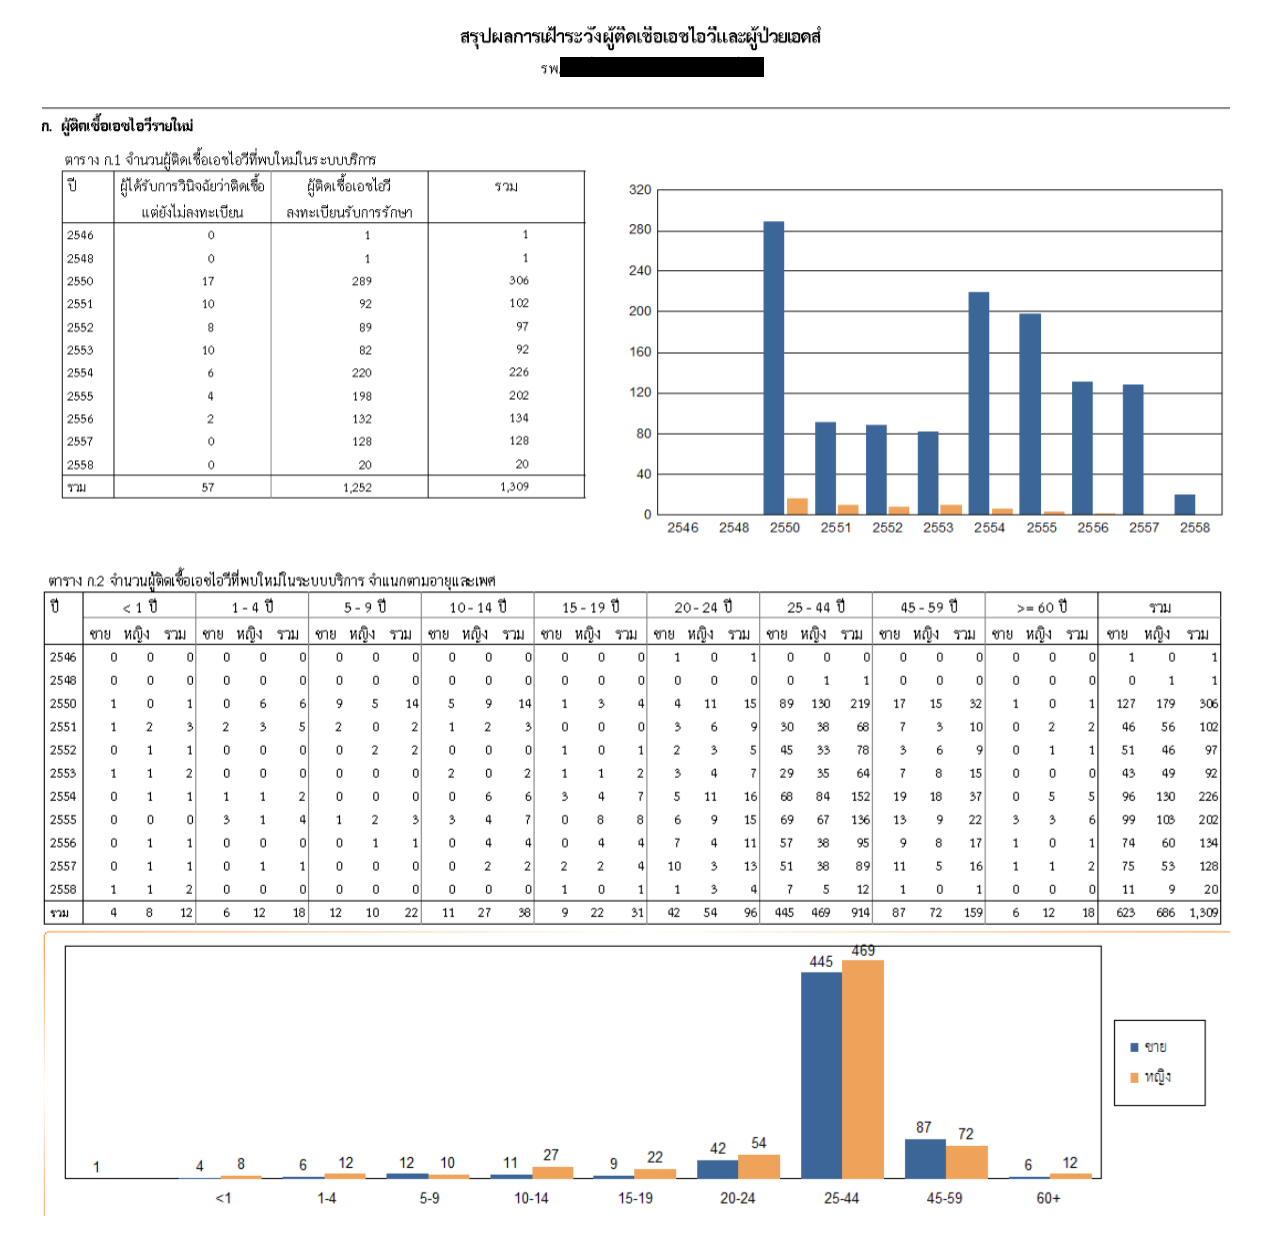
\includegraphics[width=\linewidth]{images/chapter-01/napdar-08.png}
    		\caption{NAPDAR Summary Report Page}
    \end{figure}
\FloatBarrier
	
	There are several limitations of NAP and NAPDAR. First, the data in NAP only include people who register in National Health Security Office. This means, there will be no record from the patient who does not register to National Health Security Office and the foreigners. Since Thailand has lots of foreign worker, they is one of the large portion where the budget of drug has been use. Next, the medical staff needs download each file from NAP and then upload them to NAPDAR in order to generate the report. This gives them more tasks to do. Thirdly, NAPDAR system can analyse and generate the report from the data in hospital level. It cannot generate the report of country level. This means the user of the system will not be able to see the whole picture of the situation.	


\section{Project Scope}
    
    In this project, we are going to create a solution for Bureau of Epidemiology along with other organization such as hospitals, provincial public health offices, organizations under the supervised from Ministry of Public Health (Bureau of AIDS TB and STIs, Bureau of Strategy and Policy, Information Technology and Communication Center, Bureau of Health Promotion, Office of the Permanent Secretary, Department of Medical Science), organizations under Bangkok Metropolitan Administration (Health Department, Medical Service Department), and Thailand MOPH-US CDC Collaboration. The users of the EIIS must be able to interact with the system according to their roles. Our goal is to complete the requirements as mentioned in section \ref{requirements}.
